\documentclass[a4paper,11pt]{article}
\usepackage[utf8]{inputenc}
\usepackage[russian]{babel}
\usepackage[T1]{fontenc}
\usepackage{amssymb,amsmath,graphicx}
\usepackage{caption}
\usepackage{color}
\usepackage{listings}
\usepackage[unicode]{hyperref}

\setlength{\parskip}{1ex plus 0.5ex minus 0.2ex}
\captionsetup[figure]{labelformat=empty}
\captionsetup[figure]{justification=centering}
\lstset{keywordstyle=\color{blue}\bfseries}
\lstset{extendedchars=false, language=Caml, defaultdialect=[Objective]Caml}

\author{Олег Смирнов\\
\texttt{oleg.smirnov@gmail.com}}
\date{\today}
\title{Введение в функциональное программирование -- Лекция 1. Язык F\#.
Порядок применения функции}

\begin{document}
\maketitle
\tableofcontents
\newpage

\section*{Цель лекции}
\begin{itemize}
\item Базовые понятия языка F\#
\item Нормальный и аппликативный порядок применения функции
\item Проверка и вывод типов
\end{itemize}

\section{Язык F\#}

F\# -- это мультипарадигменный язык программирования, разработанный в Microsoft
Research и предназначенный для исполнения на платформе Microsoft~.NET. F\#
наследует от языков OCaml и Haskell и сочетает функциональную парадигму с
императивными возможностями и объектной моделью .NET.

История языка началась в 2002-м году в исследовательской группе под руководством
Дона Сайма в Кэмбридже. В 2005-м вышла первая версия F\#, а уже в 2010-м он был
включён в поставку Microsoft~Visual~Studio~2010.

Базовый элемент синтаксиса F\# -- это \emph{выражение}. Примеры выражений:
\begin{lstlisting}
11
3 + 5 + 3
(1 + 2) * (3 + 4)
"Hello"
"Hello" + " World"
intToString 5
"Hello World" + 1
\end{lstlisting}

Результатом вычисления выражения является \emph{значение}. Значение будем
отделять от выражения символом =>:
\begin{lstlisting}
11 => 11
3 + 5 + 3 => 11
(1 + 2) * (3 + 4) => 21
"Hello" => "Hello"
"Hello" + " World" => "Hello World"
intToString 5 => "5"
"Hello World" + 1 - ошибка!
\end{lstlisting}

Значение получается из выражения в процессе \emph{вычисления}. Будем обозначать
один шаг вычисления символом |->. Например:
\begin{lstlisting}
    (1 + 2) * (3 + 4)
|-> 3 * (3 + 4)
|-> 3 * 7
|-> 21
\end{lstlisting}

Вычисления могут происходить последовательно, как в предыдущем примере, или
параллельно. Во втором случае, независимые друг от друга выражения вычисляются
одновременно:
\begin{lstlisting}
    (1 + 2) * (3 + 4)
|-> 3 * 7
|-> 21
\end{lstlisting}

\subsection{Типы}

Значение $"Hello~World" + 1$ не будет вычислено потому, что оно
\emph{некорректно типизировано} (ill-typed). В F\# каждое выражение имеет
\emph{тип}. Тип выражения говорит о том, какие значения могут получиться при
вычислении этого выражения и получатся ли какие-нибудь значения вообще.
Выражение \emph{корректно типизировано} (well-typed), если у него есть как 
минимум один тип. У выражение может быть более одного типа -- это называется
\emph{полиморфизм}. Хорошее описание полиморфизма и его разновидностей есть в
статье Люка Карделли ``On understanding types...''~\cite{Cardelli}.

Теория типов базируется на идеях Б. Рассела и А. Уайтхеда из работы ``Principia
Mathematica''~\cite{Russell}. Они предложили сопоставлять высказыванию
(пропозициональной функции) некоторый тип, который является его доменом или
областью определения. Иерархия, составленная из таких типов, должна была
разрешить парадоксы наивной теории множеств и послужить основанием математики.

\begin{figure}[h]
  \begin{minipage}[h]{0.49\linewidth}
    \begin{center}
        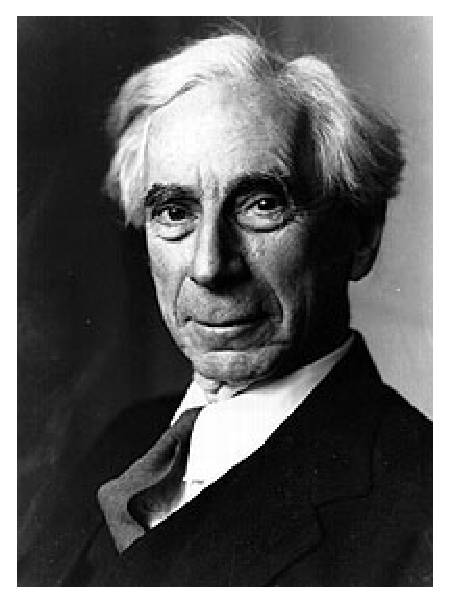
\includegraphics[height=60mm]{lecture1/russell.eps}
        \caption{Bertrand Russell\\(1872 - 1970)}
    \end{center}
  \end{minipage}
  \begin{minipage}[h]{0.49\linewidth}
    \begin{center}
      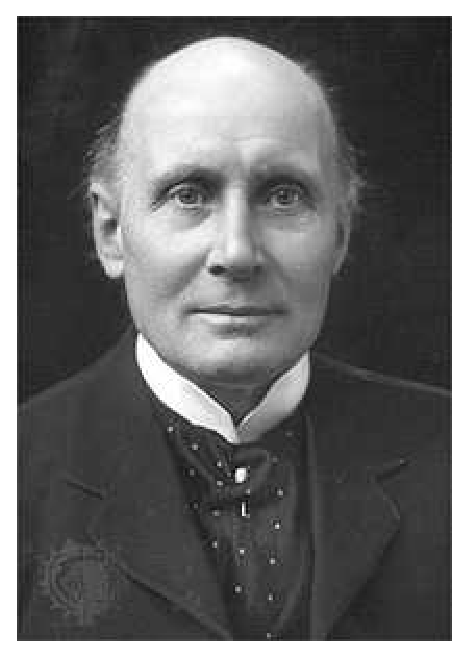
\includegraphics[height=60mm]{lecture1/whitehead.eps}
      \caption{Alfred North Whitehead\\(1861 - 1947)}
    \end{center}
  \end{minipage}
\end{figure}

Будем записывать тип выражения в формате $\langle exp \rangle : \langle type
\rangle$. Например:
\begin{lstlisting}
11 : int
"Hello" : string
"Hello World" + 1 - ошибка!
\end{lstlisting}

В общем случае, тип задаётся набором \emph{значений}, которые могут принимать
выражения этого типа и набором \emph{операций} над типом. Пример:
\begin{itemize}
\item Тип $int$
  \begin{itemize}
  \item Значения: 11, 23, \textasciitilde 42, ...
  \item Операции: +, -, $intToString$, ...
  \end{itemize}
\item Тип $string$
  \begin{itemize}
  \item Значения: $"Hello"$, $"World"$, ...
  \item Операции: +, size, ...
  \end{itemize}
\item Тип $float$
  \begin{itemize}
  \item Значения: 0.0, 2.78, 3.14, ...
  \item Операции: +, -, /, *, ... (N.B.: имена совпадают с операциями типа
    $int$, но это другие операции)
  \end{itemize}
\end{itemize}

Аналогично C\#, базовые типы являются псевдонимами для встроенных типов .NET:
System.Int32, System.String и т.д.

\subsection{Декларации}

Программа на F\# состоит из \emph{деклараций}. Рассмотрим декларацию
\emph{переменных}:
\begin{lstlisting}
  let x : int = 3 + 5 + 3
\end{lstlisting}

Переменной с именем $x$ будет сопоставлено значение выражения $3 + 5 + 3$ (типа
$int$). В общем виде переменные объявляются конструкцией 
$let~\langle var \rangle~:~\langle type \rangle~=~\langle exp \rangle$.

При вычислении последовательности деклараций $let$, вычисляется первая
декларация, а затем её значение \emph{подставляется} в следующие выражения,
в места, где упоминается соответствующая переменная. Например:
\begin{lstlisting}
  let x : int = 2 + 3
  let y : int = x + 1
  let z : int = 5 + y
\end{lstlisting}

Шаг 1:
\begin{lstlisting}
  let x : int = 5
  let y : int = x + 1
  let z : int = 5 + y
\end{lstlisting}

Шаг 2:
\begin{lstlisting}
  let x : int = 5
  let y : int = 6
  let z : int = 5 + y
\end{lstlisting}

Шаг 3:
\begin{lstlisting}
  let x : int = 5
  let y : int = 6
  let z : int = 11
\end{lstlisting}

Что произойдёт, если написать две декларации с одинаковым именем переменной?
\begin{lstlisting}
  let x : int = 5
  let x : int = 6
\end{lstlisting}

В отличии от переменных в императивной парадигме, в функциональном мире
переменные не меняют своего значения. Их скорее следовало бы называть
``постоянными''. Имя переменной \emph{связывается} с выражением (var binding).

Таким образом, во второй строке этого примера будет создано новое 
связывание между именем $x$ и выражением $6$, а старое будет ``забыто''.

Второй тип деклараций -- это декларация типов:
\begin{lstlisting}
  type coordinate = int*int
\end{lstlisting}

После этой декларации \emph{переменная типа} $row$ в программе будет означать
$int * int$. Общая форма декларации нового типа: $\langle tyvar \rangle~=~
\langle type \rangle$.

Нотация $int * int$ здесь означает пару из двух $int$. Её также можно записать
как $(int, int)$.

Область видимости в F\# -- \emph{лексическая} (она же статическая). 

\subsection{Проверка и вывод типов}

F\# -- статически типизированный язык с поддержкой определения типов. Это 
означает, что все конструкции имеют известный тип уже на этапе компиляции, а не
на этапе выполнения программы.

Алгоритм проверки типов упрощённо похож на вывод доказательства, где типы
элементарных выражений -- это аксиомы, а операции -- это теоремы (правила 
вывода). Например, аксиомы:
\begin{lstlisting}
  23 : int
  "Hello" : string
\end{lstlisting}

Правила вывода:
\begin{lstlisting}
  <exp1> + <exp2> : int если <exp1> : int и <exp2> : int
  <exp1> + <exp2> : string если <exp1> : string и <exp2> : string
\end{lstlisting}

Тогда $5 + 3 * 2 : int$, т.к. $5 : int$ -- аксиома и $3 * 2 : int$, т.к.
$3 : int$ и $2 : int$ -- аксиомы.

Кроме того, F\# -- язык со строгой типизацией. Это означает, что в выражениях
отсутствует неявное приведение типов. Например, выражение $0.1 + 1$ вызовет
ошибку компиляции, т.к. операция $+$ определена для двух $int$ или двух $float$, но
не для $float$ и $int$.

\subsection{Функции}

Как и в других языках, функция в языке F\# имеет имя, может иметь параметры и 
принимать аргументы, а также функция имеет тело. В языке F\# функции являются
\emph{объектами первого порядка}, т.е. могут возвращать функции и принимать
функции в качестве аргумента.

Функции определяются с помощью ключевого слова $let$. Формат декларации в
общем виде: $let \langle func \rangle~\langle arg \rangle~=~\langle body
\rangle$. Например, функцию $f(x) = 3*x + 2$
можно определить как:
\begin{lstlisting}
  let f (x : int) : int = (3*x) + 2
\end{lstlisting}

В случае, когда функции необходимо рекурсивно вызывать себя, в определение
добавляется ключевое слово $rec$. Пример -- функция вычисления факториала:
\begin{lstlisting}
  let rec fact n =
    match n with
      | 0 -> 1
      | _ -> n * fact (n - 1);;
\end{lstlisting}

\subsection{Функциональный тип}

Тип функции определяется как $\langle type1 \rangle \rightarrow \langle type2 
\rangle$, где $\langle type1 \rangle$ -- это тип аргумента, а $\langle type2
\rangle$ -- тип возвращаемого значения. Например, тип функции из первого примера
будет $int \rightarrow int$.

Как быть с функцией, у которой количество аргументов превышает единицу? 
Например, функция суммы:
\begin{lstlisting}
  let sum a b = a + b
\end{lstlisting}

Её тип будет $int \rightarrow int \rightarrow int$ или же $int \rightarrow (int 
\rightarrow int)$. Таким образом исходную функцию можно рассматривать как
как функцию от одного параметра типа $int$, которая возвращает другую функцию
типа $int \rightarrow int$. Всякая функция с более чем одним аргументом 
может интерпретироваться как функция от первого аргумента, возвращающая функцию
от оставшихся при фиксированном значении первого. 

Этот приём функционального программирования называется \emph{каррированием} или
\emph{каррингом} в честь математика и логика Хаскелла Карри.

\begin{figure}[h]
    \begin{center}
        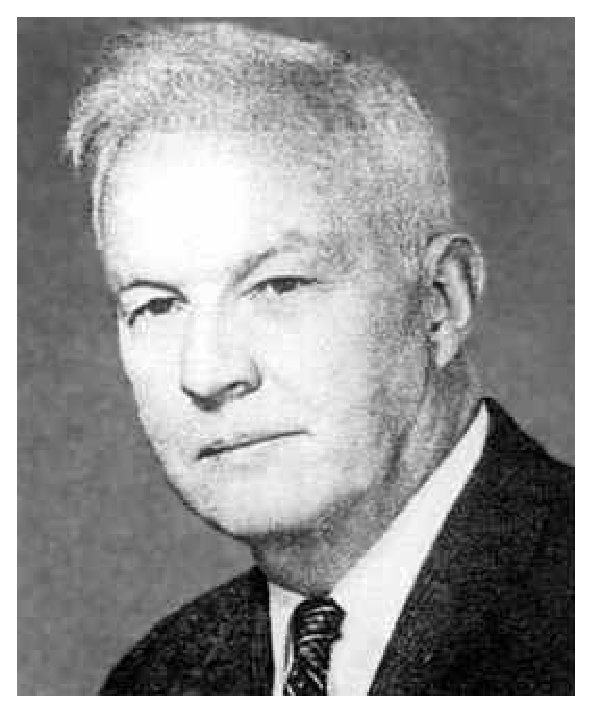
\includegraphics[height=60mm]{lecture1/curry.eps}
        \caption{Haskell Curry\\(1900 - 1982)}
    \end{center}
\end{figure}

Благодаря выводу типов, тип функции и типы аргументов во многих случаях могут
быть опущены.

\subsection{Применение и его порядок}

Главная операция для функции -- это \emph{применение} -- подстановка аргументов
в тело функции:
\begin{lstlisting}
    f 3
|-> (3 * 2) + 2
|-> 6 + 2
|-> 8
\end{lstlisting}

Есть несколько возможных порядков вычисления:
\begin{itemize}
\item aппликативный -- самый ``естественный'' порядок, при котором аргументы
функции полностью вычисляются до её вызова. Такой порядок используется в
большинстве языков программирования
\item нормальный -- порядок, при котором аргументы функции начинают вычисляться
только тогда, когда в них возникает необходимость
\item ленивый -- вариант реализации нормального порядка, при котором не
происходит дублирования вычислений
\end{itemize}

Для примера определим функцию $double$:
\begin{lstlisting}
  let double x = x + x
\end{lstlisting}

Пример аппликативного порядка:
\begin{lstlisting}
    double (double 5)
|-> double (5 + 5)
|-> double 10
|-> 10 + 10
|-> 20
\end{lstlisting}

Пример нормального порядка:
\begin{lstlisting}
    double (double 5)
|-> (double 5) + (double 5)
|-> 10 + 10
|-> 20
\end{lstlisting}

В F\# есть поддержка ленивого порядка редукции с помощью ключевого слова $lazy$.
Порядки редукции и ленивые вычисления будут подробно рассмотрены во втором
семестре курса.

\nocite{*}
\bibliographystyle{alpha}
\bibliography{lecture1}
\end{document}
